%%%%%%%%%%%%%%%%%%%%%%%%%%%%
\subsection{Эффект Казимира}

Квантовые флуктуации могут привести и к многим другим явлениям. Их влияние на, казалось бы, неквантовые объекты было теоретически показано Хендриком Казимиром~\cite{Casimir.van-der-Waals}. 
Он рассматривал взаимодействие нейтрального атома с идеально проводящей стенкой и получил асимптотические выражения для энергии при расстояниях между телами $l\to0$ и $l\to\infty$. 
Результат при $l\to0$ не вызывает удивления и даже совпадает с ответом для классического потенциала взаимодействия наведенного диполя $E \sim 1/R^3$. 
Однако при $l\to\infty$ возникает дополнительный множитель, приводящий к зависимости $E \sim 1/R^4$. 
Более того, численный множитель в этой пропорциональности содержит константу Планка, что говорит о чисто квантовой природе явления. 
Этот результат был получен при рассмотрении релятивистских (то есть с учетом запаздывания) квантовых сил ван-дер-Ваальса. 
Позже Казимир также получил аналогичный результат для идеально проводящих пластин, рассматривая разницу в энергии вакуума, вносимую их присутствием~\cite{Casimir.vacuum}. 
До сих пор не вполне понятна связь квантовых флуктуаций и сил ван-дер-Ваальса, поэтому некоторые теоретики считают рассмотрение энергии вакуума неправильным подходом, который, как это было с атомом водорода у Бора, случайно приводит к верному результату. 

Вкратце повторим рассуждения Казимира касательно энергии вакуума. Рассмотрим пространство внутри куба с достаточно большой стороной $L$. Параллельно переместим одну из сторон куба близко к противоположной и обозначим новое расстояние между ними $d\ll L$. 
В электродинамике гамильтониан, содержащий поле фотонов, приводится к интегралу бесконечного числа гармонических осцилляторов, поэтому энергию вакуума можно записать как 
$E = \sum\limits_\vec{k} \frac{1}{2} \hbar\omega(\vec{k}),$
где суммирование производится по всем возможным волновым векторам. Несмотря на то, что эта величина сама по себе, являясь бесконечной, не несет физического смысла, ее изменение определено и может быть интерпретировано как энергия взаимодействия. Для идеально проводящих пластин граничные условия зануляют тангенциальную часть напряженности на всех гранях, поэтому энергия взаимодействия
\begin{equation}
\Delta E = \frac{\hbar c}{2}\sum\limits_{n_x, n_y, n_z} \left(
\sqrt{\frac{\pi^2}{L^2}\,n_x^2 + \frac{\pi^2}{L^2}\,n_y^2 + \frac{\pi^2}{d^2}\,n_z^2} \ - \ 
\sqrt{\frac{\pi^2}{L^2}\,n_x^2 + \frac{\pi^2}{L^2}\,n_y^2 + \frac{\pi^2}{L^2}\,n_z^2}
\right).
\label{eq:dEvacuum}
\end{equation}
Эта сумма все равно расходится, поэтому необходимо как-то ограничить каждое~$n$. Благо, на это есть физическая причина: для достаточно больших частот никакая реальная поверхность не будет препятствием, поэтому перемещение пластины не повлияет на вклад больших волновых векторов в энергию вакуума. Ограничивать мы должны не $n$, а $k$. Обозначим наибольшее значение $k$ за $\Lambda$. Тогда~(\ref{eq:dEvacuum}) переписывается в виде 
\begin{equation}
\Delta E = \frac{\hbar c}{2}\sum\limits_{n_x, n_y}\left(
\sum\limits_{n_z=1}^{\Lambda d/\pi} \sqrt{\frac{\pi^2\,(n_x^2 + n_y^2)}{L^2} + \frac{\pi^2}{d^2}\,n_z^2} \ - \ 
\sum\limits_{n_z=1}^{\Lambda L/\pi} \sqrt{\frac{\pi^2\,(n_x^2 + n_y^2)}{L^2} + \frac{\pi^2}{L^2}\,n_z^2}
\right).
\label{eq:dEvac.trimmed}
\end{equation}
Не углубляясь в способы взятия таких сумм, заметим, что несмотря на гораздо большее слагаемое $1/d^2 \gg 1/L^2$ под корнем в первой сумме, число слагаемых во второй значительно больше, что пересиливает малость $1/L$. В результате изменение энергии будет отрицательным, то есть пластины будут притягиваться. 

Менее строго можно сказать, что большее расстояние $L$ позволяет большему числу волн существовать в пространстве между пластинами. А раз возможных волновых векторов больше, то больше и сумма соответствующих им частот, то есть энергия. 

\begin{figure}[t!]
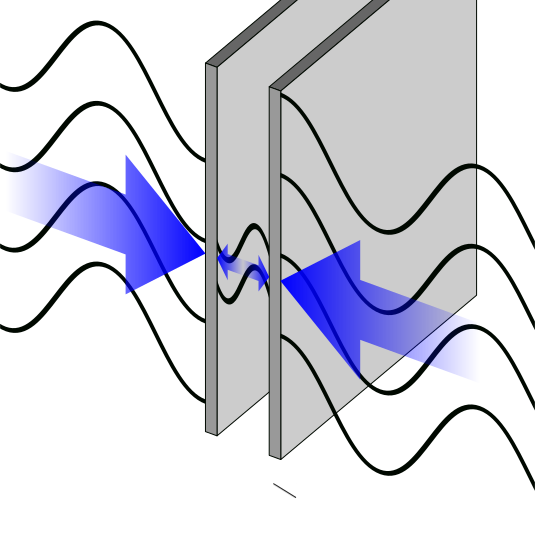
\includegraphics[width=.4\linewidth]{figs/Casimir-plates.pdf}
\caption{Силы Казимира, действующие на идеально проводящие пластины.}
\label{fig:plates}
\end{figure}

Обсудим еще один способ описать эффект Казимира в нашей системе. 
Каждая волна, как известно, оказывает давление на пластину. 
Чем ближе находятся пластины, тем меньше волн между ними может существовать, и тем слабее они будут расталкиваться. 
В то же время, пространство снаружи ничем не ограничено, волн в нем может существовать существенно больше, чем между пластинами. 
То есть снаружи на пластины действует сравнительно большая сближающая сила. 
Эта ситуация проиллюстрирована на Рис.~\ref{fig:plates}. 
Выходит, что чем меньше расстояние между пластинами, тем сильнее они притягиваются. 
На практике это играет большую отрицательную роль в системах с размерами порядка долей микрометра и меньше, поскольку детали наномеханизмов попросту слипаются в комок. 

В общем случае эффект Казимира можно представить следующим образом. 
При помещении какого-либо объекта в вакуум квантовые флуктуации изменяются, поскольку поля должны удовлетворять определенным условиям на границе вакуум-вещество. 
Энергия системы зависит от формы объекта, а значит, имеется какая-то сила. 
Существенно и удачно то, что эта сила не всегда притягивающая~\cite{General.van-der-Waals}. 
Например, идеально проводящая незаряженная сфера расталкивается изнутри за счет квантовых флуктуаций~\cite{SphericalShell}. 

%%%%%%%%%%%%%%%%%%%%%%%%%%%%%%%%%%%%%%%%
\subsection{Отталкивающие силы Казимира}

\begin{figure}
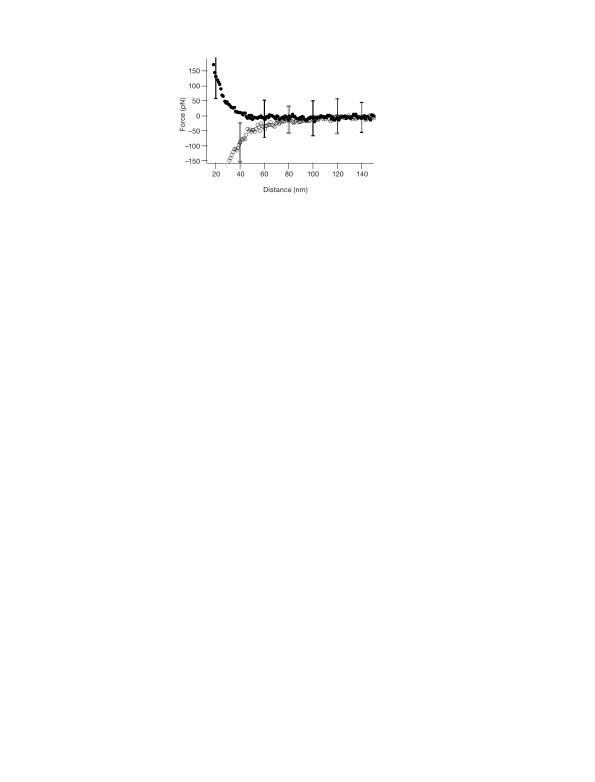
\includegraphics[width=.5\linewidth]{figs/Repulsive-graph}
\caption{Голубые (оранжевые) кружки показывают силу между золотой сферой и пластинкой из диоксида кремния (золота) в бромбензоле.}
\label{fig:rep.graph}
\end{figure}

Тема отталкивающих сил Казимира привлекает большое внимание из-за возможности применения в технологиях во-первых для достижения сверхнизкого трения, а во-вторых для избавления от упомянутых неприятностей, связанных с притягивающей силой. 
Экспериментально отталкивание наблюдалось лишь в одной конфигурации -- между двумя диэлектриками с разными проницаемостями, разделенными жидкостью с промежуточным значением проницаемости~\cite{Repulsion.firstexp}. Величина отталкивающей силы между золотом и диоксидом кремния в бромбензоле сравнима с притяжением между двумя золотыми телами, как видно на Рис.~\ref{fig:rep.graph}. Вместо двух плоских пластин в эксперименте использовались пластина и сфера, поскольку расположить пластины параллельно на таком расстоянии сложно, а сфера достаточно близка к параллельной плоскости. 

Теоретически были найдены многие подходящие системы, включая идеальные электрический и магнитный проводники~\cite{Repulsion.magnetic}, метаматериалы~\cite{Repulsion.metamaterial}. 
Однако все упомянутое довольно сложно применить на практике. 
Успехом было обнаружение отталкивания в системах с обычными проводниками: эллиптической металлической частицей и проводящей поверхностью с дыркой~\cite{Repulsion.aperture}, полубесконечными плоскостями, плоскостью и иголкой~\cite{Repulsion.plates.needle}, анизотропно поляризуемыми атомами и различными поверхностями~\cite{Repulsion.conductors}. 

\begin{figure}
\includegraphics[width=.5\linewidth]{figs/Chiral-Casimir}
\caption{Отношение сил Казимира между проводящими пластинами в хиральной среде $F_C$ и в вакууме $F_0$ в зависимости от расстояния между ними для двух значений внешнего магнитного поля.}
\label{fig:Chiral.Casimir}
\end{figure}

В общем случае было доказано, что в системах незаряженных симметрично расположенных проводников невозможно реализовать отталкивающие силы Казимира~\cite{Casimir.attr.theorem}. 
Однако этот результат основывается на отсутствии как внешних сил, так и оптической активности материалов. 
Неудивительно, что искать новые явления приходится среди специфически ведущих себя веществ. 
Совсем недавно был найден способ добиться отталкивания в хиральной среде (в которой скорости распространения лево- и правополяризованных волн не совпадают)~\cite{Repulsion.tunable}. 
Более того, вводя внешнее магнитное поле в такой системе, можно переходить от притяжения к отталкиванию, то есть, потенциально, подстраивать силу Казимира под собственные нужды. 
Необходимо, однако, заметить, что требуемые для таких манипуляций поля могут оказаться очень большими. 
Тем не менее, достичь равновесия относительно сил Казимира можно и за счет одной лишь хиральной среды, поскольку из-за нее сила существенно зависит от расстояния между объектами, как показано на Рис.~\ref{fig:Chiral.Casimir}, где $F_0 = -{\pi^2\hbar c}/{(240\,l^4)}$ -- поверхностная сила между идеально проводящими пластинами в вакууме. 
Участки с $F_C/F_0<0$ соответствуют отталкиванию. 
Как видно, существуют и устойчивые точки равновесия. 


\subsection{Вывод}

Изучение, казалось бы, простой из-за пустоты среды существенно осложняется квантовыми эффектами, которые находят подтверждение в эксперименте. 
Относящийся к изложенным темам вакуум квантовой электродинамики не является единственным.
Все взаимодействия могут привести к образованию виртуальных частиц, а значит, и квантовым флуктуациям. 
Поляризация вакуума глюонами, способными рождать друг друга переносчиками сильного взаимодействия, приводит к асимптотической свободе кварков и их конфайнменту. 
Фундаментальным теоретическим вопросом уже много лет остаются гравитационные квантовые флуктуации, предположительно приводящие к флуктуациям метрики пространства-времени, ее нелокальности и образованию виртуальных черных дыр. 

Очередной загадкой является энергия вакуума, которая должна присутствовать в общей теории относительности в уравнениях Эйнштейна в виде космологической постоянной. 
Проблема заключается в том, что, согласно даже самым оптимистичным современным представлениям, включающим до сих пор не нашедшую подтверждения суперсимметрию, ее теоретическое значение на 60 порядков больше экспериментального. 

С практической точки зрения, использование энергии вакуума может предоставить технологии совершенно нового уровня. Но поиск и реализация способных на такое устройств чрезвычайно сложны. Несмотря на все прилагаемые усилия на протяжении многих десятилетий, отталкивающие силы до сих пор экспериментально наблюдались лишь в одном типе систем. 



